\documentclass[a4paper, titlepage]{article}

\usepackage[latin1]{inputenc} 
\usepackage[T1]{fontenc}
\usepackage{geometry}
\usepackage[francais]{babel}
\usepackage{graphicx}
\usepackage{verbatim}

\title{Rapport de stage}
\author{Pr'enom Nom}
\date{18 juin 2007}

\pagestyle{headings}

\begin{document}

\tableofcontent
\section{introduction}
Bonjour et bienvenue dans le rapport de CamlT'OCR, l'OCR fait par l'equipe SMK
\subsection{les membre}
\subsubsection{Louis "Zab" Forget}
J'ai toujours été très curieux , au point de parfois même partir dans tous les sens. J'ai
toujours voulu savoir comment marche les pages web. Et c'est dans cette optique que
j'ai appris à faire du HTML et du CSS en troisième. J'ai ensuite voulu savoir comment
marchent les jeux video, puis divers programmes. Il y a quelques jours je me demandais
même comment marchent les GPS qui vous indiquent la densité du trafic, ou bien
je me demandais comment marche le logiciel photoshop.
\section{Pre traitement}
\subsection{Niveau de gris}
\subsection{Filtre median}
\section{Binarisation}i
\section{la rotation}
Je me suis donc occupé de la transformée de Hough. La transformée de Hough est une technique de reconnaissance de formes inventée en 1962 par Paul Hough. Le principe qui sous-tend la transformée de Hough est qu’il existe un nombre infini de lignes qui passent par un point, dont la seule différence est l’orientation (l’angle). La transformée généralisée de Hough fonctionne sur le même principe que la transformée de Hough :Une droite peux s'ecrire de la forme r = x cos (teta) + y sin(teta).A chaque pixel noir on essay de trouver la valeur maximum de r.Cette valeure représente la droite qui aligne le plus de pixel noire.On la retient et on vote dans un tableau pour son angle associé.On refait la meme chose sur tous les pixels.L'angle qui a été le plus voté , est l'angle de rotation de l'image (moins la moitiée de l'intervalle pour pouvoir faire ressortire les angles negatifs).
\begin{figure}[hp]

	    \centering

	    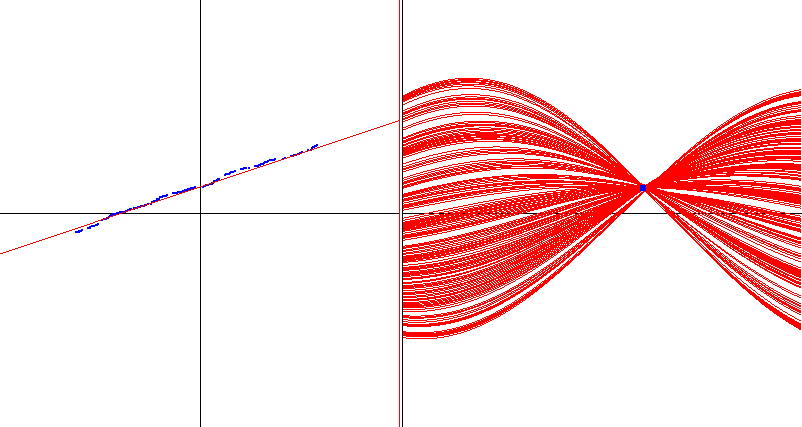
\includegraphics[width=0.80\textwidth]{hough.jpg}

	    \caption{hough}

\end{figure}

\section{le reseau de neurone}
\end{document}

